\chapter{Introduction}
\section{Quantum chromodynamics (QCD)}
The Quantum Chromodynamics (QCD) is the fundamental theory of the strong interaction.
It describes the interaction of objects that carries color charges. 
Quarks and gluons are the fundamental degrees of freedom of the theory. 
Quarks are fermions and gluons are bosons that mediate the interaction between color charges.
The QCD Lagrangian (with one flavor of quark) is,
\begin{eqnarray}
\mathcal{L} = \bar{\psi_i} \left(i\gamma_\mu D^\mu_{ij} -m \delta_{ij} \right)\psi_j - \frac{1}{4}G_{\mu\nu}^a G^{\mu\nu,a},
\end{eqnarray}
where $\psi_i$ the Dirac spinor of the quark field with color $i = 1,2,\cdot N_c$. 
\begin{eqnarray}
D^\mu = \partial^\mu - i g T^a A^{\mu, a}
\end{eqnarray}
is the covariant derivative which contains the interaction between quark field and the gluon field.
The pure gauge term involving the field tensor,
\begin{eqnarray}
G^{\mu\nu,a} = \partial^\mu A^{\nu, a} - \partial^\nu A^{\mu, a} + g f^{abc} A^{\mu,b}A^{\mu,c}
\end{eqnarray}
contains the kinematic term and the self interaction of the gluon field.
The non-linearity of the gluon self interaction comes from its non-abliaen nature, manifesting as the structure constant $f^{abc}$.
The Feynman rule for QCD is summarized as follows,
\begin{figure}
    \centering
    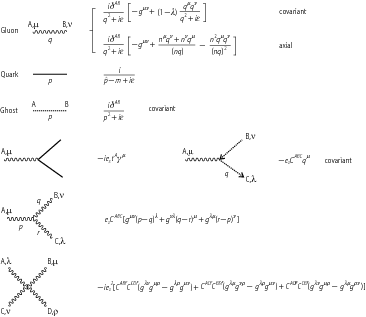
\includegraphics{qcd-feynman-rules.png}
    \caption{Caption}
    \label{fig:qcd-feynman}
\end{figure}

Due to quantum fluctuations, the coupling constant of the quantum field theory runs with the resolution, i.e., energy scale. 
In perturbation theory, the running of the strong coupling constant, characterized by the $\beta$-function, can be calculated order by order, 
\begin{eqnarray}
\frac{\partial g}{\partial \ln\mu} = \beta(g).
\end{eqnarray}
At leading order, the QCD $\beta$ function with number of colors $N_c$ and $n_f$ flavors of fermions is,
\begin{eqnarray}
\beta(g) = - \left( \frac{11}{3}N_c - \frac{2}{3}n_f \right) \frac{g^3}{16\pi^2}.
\end{eqnarray}
This $\beta$ function is negative for $N_c=3$ and realistic $n_f = 2\cdots 6$, meaning the effective coupling constant decreases with increasing energy resolution.
This feature is known as the asymptotic freedom of QCD that its interaction becomes small at asymptotically high energy.
It is the asymptotic freedom that made possible the usage of perturbation theory at high energy.
Solving which yields the leading order running coupling constant $\alpha_s = g^2/4\pi$ as a function of energy scale,
\begin{eqnarray}
    \alpha_s(\mu^2) = \frac{4\pi}{\left(\frac{11}{3}N_c - \frac{2}{3}n_f\right)\ln\left(\frac{Q^2}{\Lambda^2}\right)}
\end{eqnarray}
With the integration constant absorbed into the QCD energy scale $\Lambda$, determined by experimental measurements. 
At leading order $\Lambda \approx 200$ MeV.
Before hitting this energy scale, the coupling constant is already becoming too large for reliable perturbative calculations.
$\Lambda$ is often an estimation of the non-perturbative scale of QCD.

\begin{figure}
    \centering
    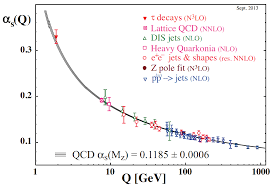
\includegraphics{alphas.png}
    \caption{Caption}
    \label{fig:alphas}
\end{figure}

At low energy $Q\sim \Lambda$ or large distance, the theory enters the non-perturbative regime. 
The coupling between color charges is so large that isolated color cannot exist alone without its strong color field constantly populating more color objects.
The color charges combined to form colorless QCD bound states known as hadrons, such as protons, neutrons and pions.
Depending on its content valance quarks (quarks that carry the net quantum number), hadrons are generally categorized as baryons and mesons.
Baryons are hadrons with three valance quarks or anti-quarks, while mesons consist of a valance quark and an anti-quark.
Besides valance quarks, hadrons are also populated with sea quarks pairs and gluons due to quantum fluctuations.
The physics of non-perturbative regime cannot be obtained from perturbative QCD and the only reliable way nowadays is lattice QCD technique where the QCD Lagrangian is discretized on a finite lattice and studied on a computer.

\section{The QCD phase diagram}
Ever since QCD is proposed to be the fundamental theory of strong interaction (and therefore nuclear physics) and the discover of asymptotic freedom, people have been questing for the phase structure of nuclear matter. 
The phase-diagram is often studied with temperature and baryon chemical potential as independent variables. 
The phase structure on the landscape of independent thermodynamic quantities such as isospin asymmetry, strangeness, etc have also attract great attentions.
Ordinary nuclear matter (nuclei) are many body bound states at zero temperature and Baryon chemical potential $\mu_B\approx 1$ GeV.
A first insight at finite temperature is that because the weakening of the coupling at high energy scale, the nuclear matter was thought to transit from hadronic matter to a system of liberated quarks and gluons, termed the quark-gluon plasma (QGP). 
Lattice QCD calculations have studied this transition at zero baryon chemical potential with physical parameters.
Figure \ref{fig:qcd_eos} quotes the results obtained from the HotQCD Collaboration.
It shows the pressure, energy density and entropy density of the 2+1 flavor QCD.
The thermodynamic quantities scaled by powers of temperature can be understood as the effect number of degrees of freedom.
The non-interacting limit (ideal gas of quarks and gluons) is denoted as the dashed lines. 
It is observed that the lattice results converges to the expectation from a hadron resonance gas model (HRG) at low temperature and smoothly transit to higher values in a narrow temperature range around the pseudo critical temperature $T_c \approx 150 $ MeV, suggesting an increase of degrees of freedom.

This transition is a cross-over type phase transition at vanishing baryon chemical potential.
At finite baryon chemical potential, the lattice QCD is faced with the fermion sign problem. But many phenomenological models and Dyson-Schwinger equations studies have suggested the existence of a first order phase transition at large $\mu_B/T$.
If such a first order phase transition exist, the coexistence line must end at some point when decreasing $\mu_B/T$, approaching the cross-over phase transition established from lattice study.
Such a point, called the critical end point (CEP), is of great interest both theoretically and experimentally.
At high enough chemical potential (density) and low temperature, another phase of nuclear matter known as the "Color Superconductor" has been proposed, where the quarks forms Cooper pairs as those found among electrons in common superconductors.

Experimentally, colliding heavy nuclei at ultra-relativistic high energies allows one to explore the high temperature region of the phase diagram.
Since 2005, the Relativistic Heavy-ion Collider (RHIC) at the Brookheaven National Laboratory (BNL) started colliding gold nuclei at 200 GeV. 
The Large Hadron Collider (LHC) started its heavy ion programs later, colliding lead nuclei at 2.76 TeV and 5.02 TeV.
A striking discovery is that, contrary to previous expectation of weakly coupled gas of quarks and gluons, there are many evidences point that the state of matter created resembles a nearly perfect fluid in the estimated temperature range of a few times of $T_c$.
This discovery reveals the strongly coupled nature of the matter produced in relativistic nuclear collisions and has been entitled the name strongly coupled quark-gluon plasma (sQGP).
The phenomenology of relativistic heavy-ion collisions is discussed in detail in the next chapter.

\begin{figure}
    \centering
    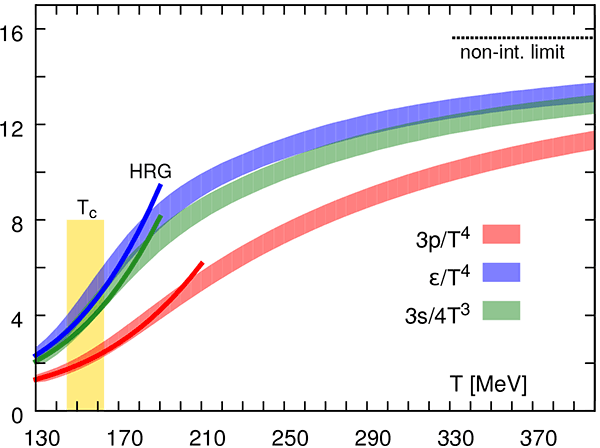
\includegraphics[width=.8\textwidth]{qcd-eos.png}
    \caption{Caption}
    \label{fig:qcd_eos}
\end{figure}

\begin{figure}
    \centering
    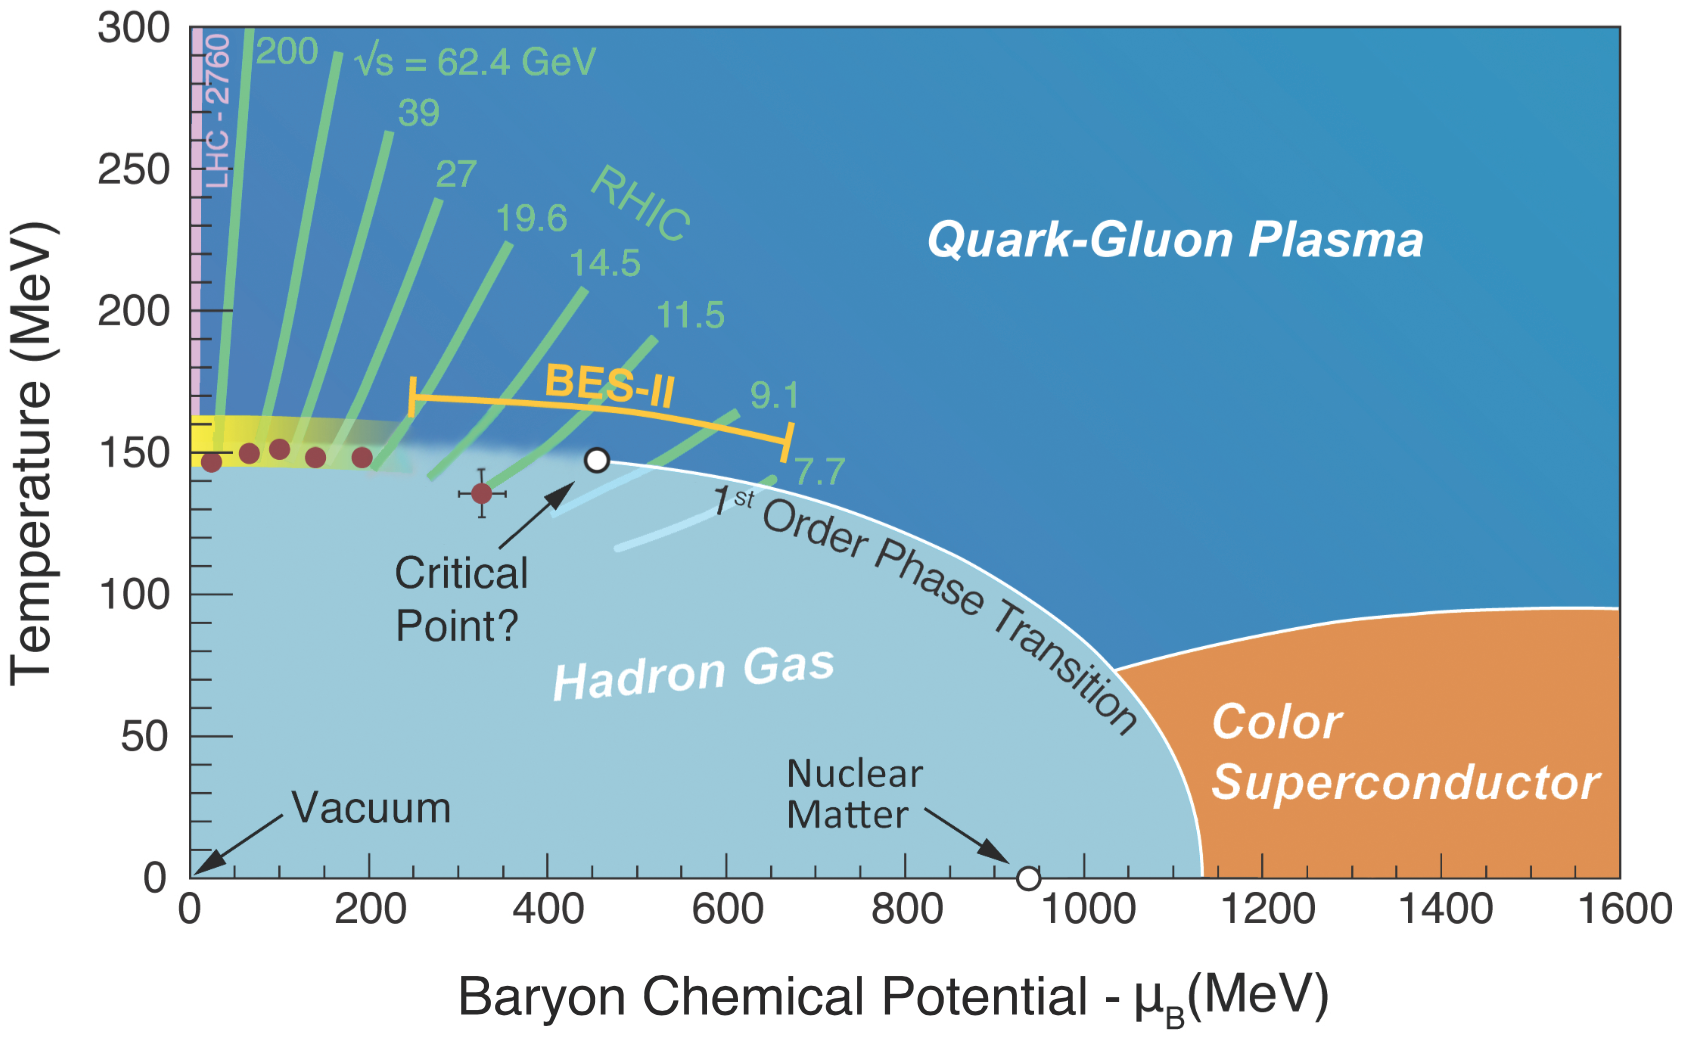
\includegraphics[width=.8\textwidth]{phase-diagram.png}
    \caption{Caption}
    \label{fig:phase-diagram}
\end{figure}


\section{Relativistic heavy-ion collision}
In recent years, the Relativistic Heavy-Ion Collider (RHIC) at Brookhaven National Laboratory and subsequently the Large Hadron Collider (LHC) at CERN have discovered a new state of matter in ultra-relativistic heavy-ion collisions, referred to as the quark-gluon plasma (QGP).
The three key observations that lead to 
the discovery of the QGP are the measured strong collective flow of bulk matter, parton recombination as manifest in constituent quark number scaling laws and jet energy-loss (i.e. jet quenching). 

The observed collective flow reveals that the bulk medium of the QGP undergoes a strong collective expansion after its initial creation.
This behavior can be explained in surprisingly great detail by models using relativistic viscous hydrodynamics.
Jet quenching refers to the strong suppression of the yield of high transverse momentum hadrons in nuclear collisions, compared to the scaled yield in proton-proton collisions where medium effects are assumed to be small.
Calculations have shown that this suppression is a consequence of jets losing energy to the hot, dense and color-deconfined medium. 

Heavy quarks (charm and bottom) are often seen as complementary probes of the QGP, but partly also belong to the category of jet observables, depending on their transverse momenta. Their large masses (compared to the prevailing temperatures generated in collisions at current heavy-ion colliders) constrain their production to early reaction times via hard perturbative Quantum-Chromodynamics (pQCD) processes. Flavor conservation ensures that the overwhelming majority of heavy quarks survive the entire reaction, allowing them to probe the full space-time evolution of the reaction.
These two features are particular attractive to theorists as these flavor-tagged particles are much easier to track in the calculations than the evolution of a full jet.
The mass also sets an additional energy scale to the problem and brings rich physics to the heavy-flavor sector.
In the high transverse momentum region, heavy quarks lose energy mainly through radiative processes connecting them to jet energy loss studies {Wicks:2007am, Djordjevic:2004nq, Xu:2014tda, Kang:2016ofv}, whereas
in the low transverse momentum region their large mass delays their thermalization, providing a window to study the equilibration process {Moore:2004tg,Riek:2010fk,Cao:2013ita}.
Heavy flavors are therefore ideal and unique probes to determine QGP properties.

The in-medium propagation of heavy quarks is often studied in a kinetic approach that is linearized with respect to the heavy quark distribution function and the medium particle distribution function is assumed to be thermal, obtained from hydrodynamic models.
The linearization implies that any effects of the heavy quark interactions on the medium are neglected.

The linearized Boltzmann transport equation and the Langevin equation are both widely used linearized models but make different assumptions regarding the nature of the interaction and thus often focus on different regimes in the heavy quark phase space {Auvinen:2009qm,Cao:2016gvr, Cao:2017hhk, PhysRevD.37.2484, Moore:2004tg}.
The linearized Boltzmann transport equation is based on elementary scattering processes that can be directly calculated, e.g. via pQCD.
However, calculations in the presence of a medium are extremely complicated even at leading order {Arnold:2002zm}.
Also, the pQCD processes are often plagued by soft divergences that need to be regulated by a medium scale proportional to temperature. Moreover, at current collision energies the relevant temperature is not high enough which creates ambiguities for the pQCD calculation through the scale dependence of the strong coupling constant $\alpha_s$.

The Langevin equation takes a different approach: 
it assumes that heavy quark receives frequent but soft momentum kicks from the medium, making a statistical description of the interaction possible -- in terms of ``drag" and ``diffusion" coefficients.
These transport coefficients encode the first and second moments of the momentum-exchange rate but are agnostic to further details of the elementary processes and medium properties.
There are efforts to calculate these transport coefficients in various approaches including lattice QCD {Moore:2004tg,CaronHuot:2008uh, Gossiaux:2008jv,He:2012df,Riek:2010fk,vanHees:2007me,Scardina:2017ipo,Ding:2012sp,Banerjee:2011ra,Francis:2015daa}. Our group has taken a complementary approach, using experiment data to calibrate our Langevin based transport model to measured observables and thus extract the transport coefficients directly from data via a Bayesian analysis {Xu:2017obm}. The drawback of this approach is that it does not in itself provide a fundamental understanding of the interaction mechanism but can only provide guidance to direct calculations of the transport coefficients in terms of compatibility to experimental observation.

In this work, we propose to combine the strengths of the linearized Boltzmann equation approach with that of the Langevin equation to develop a hybrid transport model for the evolution of heavy quarks in a QGP medium.
In this hybrid model, called {\tt Lido} ({\bf Li}nearized Boltzmann with {\bf d}iffusion m{\bf o}del),  the heavy quarks scatter off medium particles described by a linearized Boltzmann equation with pQCD matrix elements (the scattering component), and between scatterings propagate according to a Langevin equation (the diffusion component) with empirical temperature- and momentum-dependent transport coefficients to describe the soft non-perturbative components of the interaction missing from the above scattering picture.
Both elastic and inelastic scatterings are included in the scattering component with the soft divergence screened by a Debye mass $m_D$ and the Landau-Pomeranchuk-Migdal (LPM) effect taken into account effectively.
The scattering process inside a medium is a multi-scale problem that includes a momentum transfer scale $Q$ and a medium scale that is proportional to the temperature $\mu\pi T$.
The QCD coupling constant has a scale dependence that we choose to be the maximum of $Q$ and $\mu\pi T$, which means the typical scale of an in-medium process is cut off by the medium scale.
The details of the running coupling constant we have utilized can be found in Appendix \ref{appendix:alphas}.
The medium scale parameter $\mu$ is the only parameter in the scattering component and we assume it encodes the uncertainty in the pQCD matrix-element approach in our models.
The diffusion component has several parameters depending on the way in which transport coefficients are parametrized. 
The idea is to include non-perturbative contributions in terms of these transport coefficients.
For future studies, we will also consider absorbing small-momentum-transfer elastic pQCD scatterings and the associated radiation into a radiation-improved Langevin equation component of the model.
We would like to point out that a rigorous separation of matrix-element based scattering and diffusion has been proposed for the study of light parton jet energy loss up to next-to-leading order in pQCD {Ghiglieri:2015ala}.
In our study, we don't require the diffusion component to be perturbative in nature.

All parameters of the model will be calibrated to data using Bayesian inference {Novak:2013bqa,Bernhard:2015hxa}.
This approach takes experimental uncertainties into account and provides the probability distributions for all model parameters given the experimental data.
The Bayesian technique is particularly useful for focusing on a subset of parameters such as the transport coefficients.
It allows the marginalization over all other parameters and computes the probability distribution for the parameters of interest. 
The marginalization provides a parameter range that is not only preferred by the experiments, but also already includes uncertainties in the other model parameters.
Therefore the Bayesian technique reveals what actually can be learned from the data, considering both experimental accuracy and model uncertainties.
The Bayesian methodology has been successfully applied to the extraction of initial condition and bulk transport coefficients of the soft QGP medium {Novak:2013bqa, Pratt:2015zsa, Bernhard:2015hxa, Bernhard:2016tnd, Auvinen:2017fjw} and to the heavy quark sector for the extraction of the heavy quark momentum diffusion parameter $\hat{q}$ using a radiation improved Langevin equation {Xu:2017obm, Cao:2013ita}.
In this work, we shall perform a likewise extraction of the heavy quark transport properties using the proposed {\tt Lido} model and compare with previous calculations to see how the results dependent on the use of different transport approaches.


Heavy ion collisions are major experimental tools to study nuclear matter at high energy density.
In this chapter, I shall introduce the basics of collider physics to be used extensively in the rest of this thesis. 
This includes concepts and terminologies from both hadron and nuclear collisions. 
Then, I will discuss on the status experimental observations and the theoretical understandings and challenges.

High energy colliders are important tools for high energy physics study. 
Hadron such as protons and anti-protons and various nuclei are accelerated to ultra-relativistic energies and collide, depositing a huge amount of energy in the center-of-mass (CoM) frame for particle production.

It is advantages think of the relavistic collision in a new set of coordinates that is related to the Cartesian coordinates by,
\begin{eqnarray}
x_\perp &=& x_\perp\\
\tau &=& \sqrt{t^2 - z^2}\\
\eta_s &=& \frac{1}{2}\ln\frac{t+z}{t-z}
\end{eqnarray}
where the $z$ direction aligns with the accelerated beam direction.
$\tau$ is called the ``proper time" and $\eta_s$ called the space-time rapidity.
One advantage of using this set of coordinates is that $\tau$ and $\eta_s$ transforms much simpler than $t$ and $z$ under Lorentz boost ($\beta_z$) in the beam direction,
\begin{eqnarray}
\tau' &=& \tau,\\
\eta_s' &=& \eta_s + \frac{1}{2}\ln\frac{1+\beta_z}{1-\beta_z}
\end{eqnarray}
Similarly, for momentum the transverse mass is defined as $m_T^2 = m^2 + p_T^2 = E^2 - p_z^2$ and the rapidity is $y = \frac{1}{2}\ln\frac{E+p_z}{E-p_z}$.
Besides, pseudo-rapidity is often used experimentally,
\begin{equation}
    \eta = \frac{1}{2}\ln\frac{|p|+p_z}{|p|-p_z} = \frac{1}{2}\ln\frac{1+\cos\theta}{1-\cos\theta}
\end{equation}
It has the merits that it is directly related to the polar angle of final state particles and that it is an approximate for rapidity when the transverse mass is negligible.

In the center-of-mass frame of the colliding nuclei, due to the Lorentz contraction in the beam direction, the nuclei ``shrinks" in the $z$ direction by the factor $\gamma = (1-v^2)^{-1/2} = E/M$. 
For example, at top RHIC energy the energy per nucleon in the center-of-mass frame is 100 GeV, and the rest mass of nucleon is about 1 GeV, yielding a contraction factor of 100. 
At top energy for Pb+Pb collision at the LHC, this factor can be as large as 2500.
Therefore, the high energy nuclei ``look like pancakes" with transverse spatial extend about the nucleus radii, but a highly concentrated profile in the beam direction $\delta z \sim 2R/\gamma$.
As the result the penetration of the colliding nuclei happened almost instantaneously compared transverse dynamics.
Energy is deposited in the overlapped area and entropy is rapidly produced, creating an expanding fireball in the middle while the nuclear remnants recede.
This highly excited fireball of fields undergoes complex dynamics and cools down.
Eventually, it reaches a point that the strong fields is again confined into hadrons. The hadrons may decay into other hadrons, photons and lepton, or free-stream into the detectors.

Nuclei are extended objects, and collision geometry can fluctuate from complete overlap (small impact-parameter) to peripheral interaction (large impact-parameter).
It is impossible to determine precisely the impact-parameter by analyzing the final state. 
However, an approximate handle on the the collision geometry is the ``centrality" meter. 
Centrality can be defined in different ways at different kinematic cuts, but the idea is to reflect the nuclear collision geometry by the amount of particle production activity.
It is not hard to anticipate the number of charged particles produced or the total transverse energy observed by the detector increases as the impact parameter decreases, up-to fluctuations.
These approximate correspondence between centrality measure and impact-parameter gives a powerful handle on selecting events with particular nuclear collision geometry.


It is our goal to understand this state of highly excited nuclear matter and probe its properties.
Experimentally, it is found that produced charged particles has a wide distribution in rapidity / pseudo-rapidity with a plateau around the middle rapidity $\eta = 0$.
The formation of such a plateau is also observed in proton proton collision and can be explained by the way QCD produces particles.
The transverse momentum $p_T$ spectra of produced particles are very steep, meaning that the majority of particles produced in one event are relatively soft (involving small $p_T$) with $p_T \lesssim 3$ GeV.
These particles forms the ``soft" observables. 
Very occasionally, particles with large transverse momentum ($p_T\gtrsim 10$ GeV) are produced, and there are referred to as the ``hard" particles.
By uncertainty principal, these hard particles can only be produced in the initial collisions on a time scale $\delta t \sim 1/p_T$.
Therefore, a hard process can only be produced at the very beginning of the nuclear collision and interacts with the nuclear medium that surrounds it.
Due to the large $p_T$ and relatively small coupling constant, the production of these hard particles can be studied in a perturbative framework.
The interaction with the medium modifies the initial production and leaves finger prints of the nuclear matter properties in the hard observables. 
So, these hard particles can be used as self-generated probes of the system.

In the following sections, I shall introduce the key observations from soft physics and the current ``standard model" for describing the bulk medium evolution.
This focus on particularly the anisotropic flows and the hydrodynamic based modeling.
After that I devote a section to discuss one of the remaining challenge of the medium evolution: the initial stage, and explain my contribution to this problem.
The rest of this chapter will be focusing on the hard probes, including the production in hadronic collision, the jet quenching phenomenon in nuclear collisions, and finally introduce the main focus of this thesis: heavy-flavors as hard probes.

\subsection{Anisotropic flows and QGP transport coefficient}
One of the most striking discovery from RHIC and LHC heavy-ion program is the large anisotropic flows in the final charged particle distribution function.
Decomposing the invariant spectra of particle production into Fourier series of the azimuthal angle,
\begin{eqnarray}
E\frac{dN}{p_T dp_T d\phi dy} = \frac{1}{2\pi}\frac{dN}{p_T dp_T dy}\left(1 + \sum_{n=1}^{\infty}v_n(p_T)\cos\left[n(\phi-\Psi_n)\right]\right).
\end{eqnarray}
The first term in the expansion is azimuthal angle averaged yield.
The terms in the sum expands the angular dependence. 
The $n=1$ term is a modulation of the center of mass, which we neglect by virtue of symmetry at mid-rapidity.
From $n=2$, a non-zero $v_n$ characterize the anisotropy in momentum-space of various order.
If the particle production in high energy nuclear collisions is simply an independent sum of elementary nucleon binary collisions, then the anisotropy would be zero after averaging over many events. 
However, experiments observe a surprisingly larger elliptic flow ($v_2$) in Au+Au collisions and later in Pb+Pb collisions.
Higher order flows harmonics and in particular odd order $v_n$ were discovered later.
The large anisotropic flow suggests a substantial role of final state interaction among excitations after the initial production.
The ideal hydrodynamic model that assumes immediate realization of local thermal equilibrium, i.e., strong and frequent final state interaction, explains elliptic flow very well.
In the hydrodynamic picture, the deformed fireball created in non-central nuclear collision and expands hydrodynamically. 
The initial spatial anisotropy results in a pressure gradient differences in the long- and short-axis directions.
The higher pressure gradient in the short axis direction drives a fast expansion than the perpendicular direction, explaining the quadrupole azimuthal modulation.
The existence of odd order harmonics seemed odd but was explained by the simple idea that the nuclear wave function fluctuates on such a short time scale. 
The randomized nucleon positions results in non-zero odd-order initial eccentricities that drives the respective anisotropic flows.
Improving ideal hydrodynamics, relativistic viscous hydrodynamics was developed to include off-equilibrium effects, which includes important QCD transport properties as the shear and bulk viscosity.
The QGP shear viscosity and bulk viscosity are of fundamental importance. 
The shear viscosity to entropy ratio is related to the stong / weak coupling nature of the relevant dynamics. 
The bulk viscosity is shown to be directly replaced to the QCD trace anomoly and scale-invariance breaking.
Study has shown that anisotropic flows are sensitive probes of the QCD shear viscosity.
Stronger constraining power for both shear and bulk viscosities can be achieved by global fitting to a variety of bulk observables.
It is found that small but non-vanishing values of shear- and bulk-viscosity-to-entropy ratio is needed to quantitatively describe the data quantitatively.

\subsection{``Standard model" of bulk evolution}


\subsection{Hard probes}

\subsection{Jet quenching}

\subsection{Physics of heavy-flavors}